\section{Discussion} \label{chap:discussion}
% Employment in affected sectors in 2014

% Ex ante
% Knabe Schob 2008: -0.84M
% Ragnitz  Thum 2007: -1.1M
% Bachmann 2008: -1.2M
% Bauer 2009: -0.85M
% Muller Steiner 2010: -140K

% Ex post
% Caliendo 2017: -0.3% / 78K in regular, 2.4% / 180K in mini-jobs / regional variation in bite
% Bossler 2016: -1.9% / 60K / survey question on having a worker <MW / parallel trend is questionable
The small but negative overall effect on employment (-1.1\%) is broadly in line with other studies of the German minimum wage. \citet{Bossler2016} finds a reduction in employment of 1.9\% based on the IAB Establishment Panel 2011-2015 which included a question on whether the firm had employees earning less than €8.50. The larger effect size may be due to a cleaner treatment-control distinction, although this comes at the cost of reduced similarity in the pretreatment period, which could also partially drive their result. The approach in \citet{Caliendo2018le} is more similar to ours, but where we get the identifying variation from sectoral differences, they use geographical differences in the minimum wage ``bite''. They find a much smaller effect on regular employment (-0.3\%), but a significantly larger effect for mini-jobbers (-2.9\%).\footnote{Mini jobs are limited to a monthly pay of €450 per month and are tax free, although the employer still has to pay social security contributions.} This differential impact on regular versus marginal employment is also present in \citet{Garloff2016}, who uses region-age-gender variation in the minimum wage bite to identify the employment effect. They find that the number of mini jobs lost balance out the gains in regular employment, suggesting there might be a shift from one form to the other.

In order to compare our results to the numerous ex ante predictions, we first need to convert the relative employment loss to an absolute number of jobs foregone. In 2014, Germany counted 38 million employees.\footnote{Source: Destatis. Includes both regular and marginal employment, but exludes interns and the self-employed.} Of those, 4.8 million were employed in an affected sector. Multiplying this number by our semi-elasticity, our back-of-the-envelope estimate suggests 54 000 jobs were lost due to the national minimum wage. This represents a mere 0.14\% of total employment and is in line with the previously mentioned ex-post studies. It is however far below most ex-ante predictions. Those were generally clustered around a million jobs lost (\citealp{Knabe2008}: 0.84M; \citealp{Ragnitz2007}: 1.1M; \citealp{Bachmann2008}: 1.2M; \citealp{Bauer2009}: 0.85M), with the notable exception of \citet{Muller2010}, who predicted a more conservative 150 000 job losses. A potential explanation for this large discrepancy is that those ex-ante studies were performed at a time when German unemployment was twice as high (10\% vs 5\% in 2014) and estimated wages in the bottom decile were remarkably lower \citep{Muller2013}.

Next to the overall effect, we also find evidence of heterogeneous impacts across sectors, as shown by Figure \ref{fig:sectorSplit}. The bars represent the average treatment effect per sector, split for West and East Germany (resp. dark and light grey). The number of treated firms is shown on the left. Not only are some sectors more strongly affected, a handful appear to have profited from the minimum wage introduction. Most notably, the restaurant and fastfood sector (NACE 56) saw robust (and as shown in Table \ref{table:mainResults}, statistically significant) employment growth after the minimum wage introduction. 

There are multiple potential explanations. Restaurant prices are relatively volatile, changing by 2-3\% each year even in low general inflation periods.\footnote{Source: Destatis, Verbraucherpreisindex.} This makes it easier to pass on cost increases to the consumer without suffering short-term competitive losses. There is some US evidence for this, e.g. \citet{Allegretto2018} show that restaurants in San Jose, CA passed on to costumers nearly the entire cost increase due to a 25\% hike in the local minimum wage. A complementary explanation is the presence of a positive product demand effect if increased earnings are spent on food away from home. Indeed, 2015 saw a 12\% decline in the number of people who \emph{never} eat out as well as an increase in the number of people eating out \emph{often}.\footnote{Source: Statista, \url{https://www.statista.com/statistics/561124/eating-out-frequency-germany/}, accessed April 2018.} This might put the results from American studies in perspective, which are generally limited to studying either restaurants or teenagers.\footnote{Due to the low level of the US minimum wage, no other meaningful sectors employ considerable numbers of potentially affected workers.} If the restaurant sector there can adapt to higher minimum wages in a similar fashion, it can be dangerous to extrapolate the lack of disemployment effects found in that sector (e.g. \citealp{Dube2010}, \citealp{Allegretto2011}) to the wider economy.

\begin{figure}[htbp]
    \centering
    \caption{Average treatment effect by sector (split East/West Germany)}
    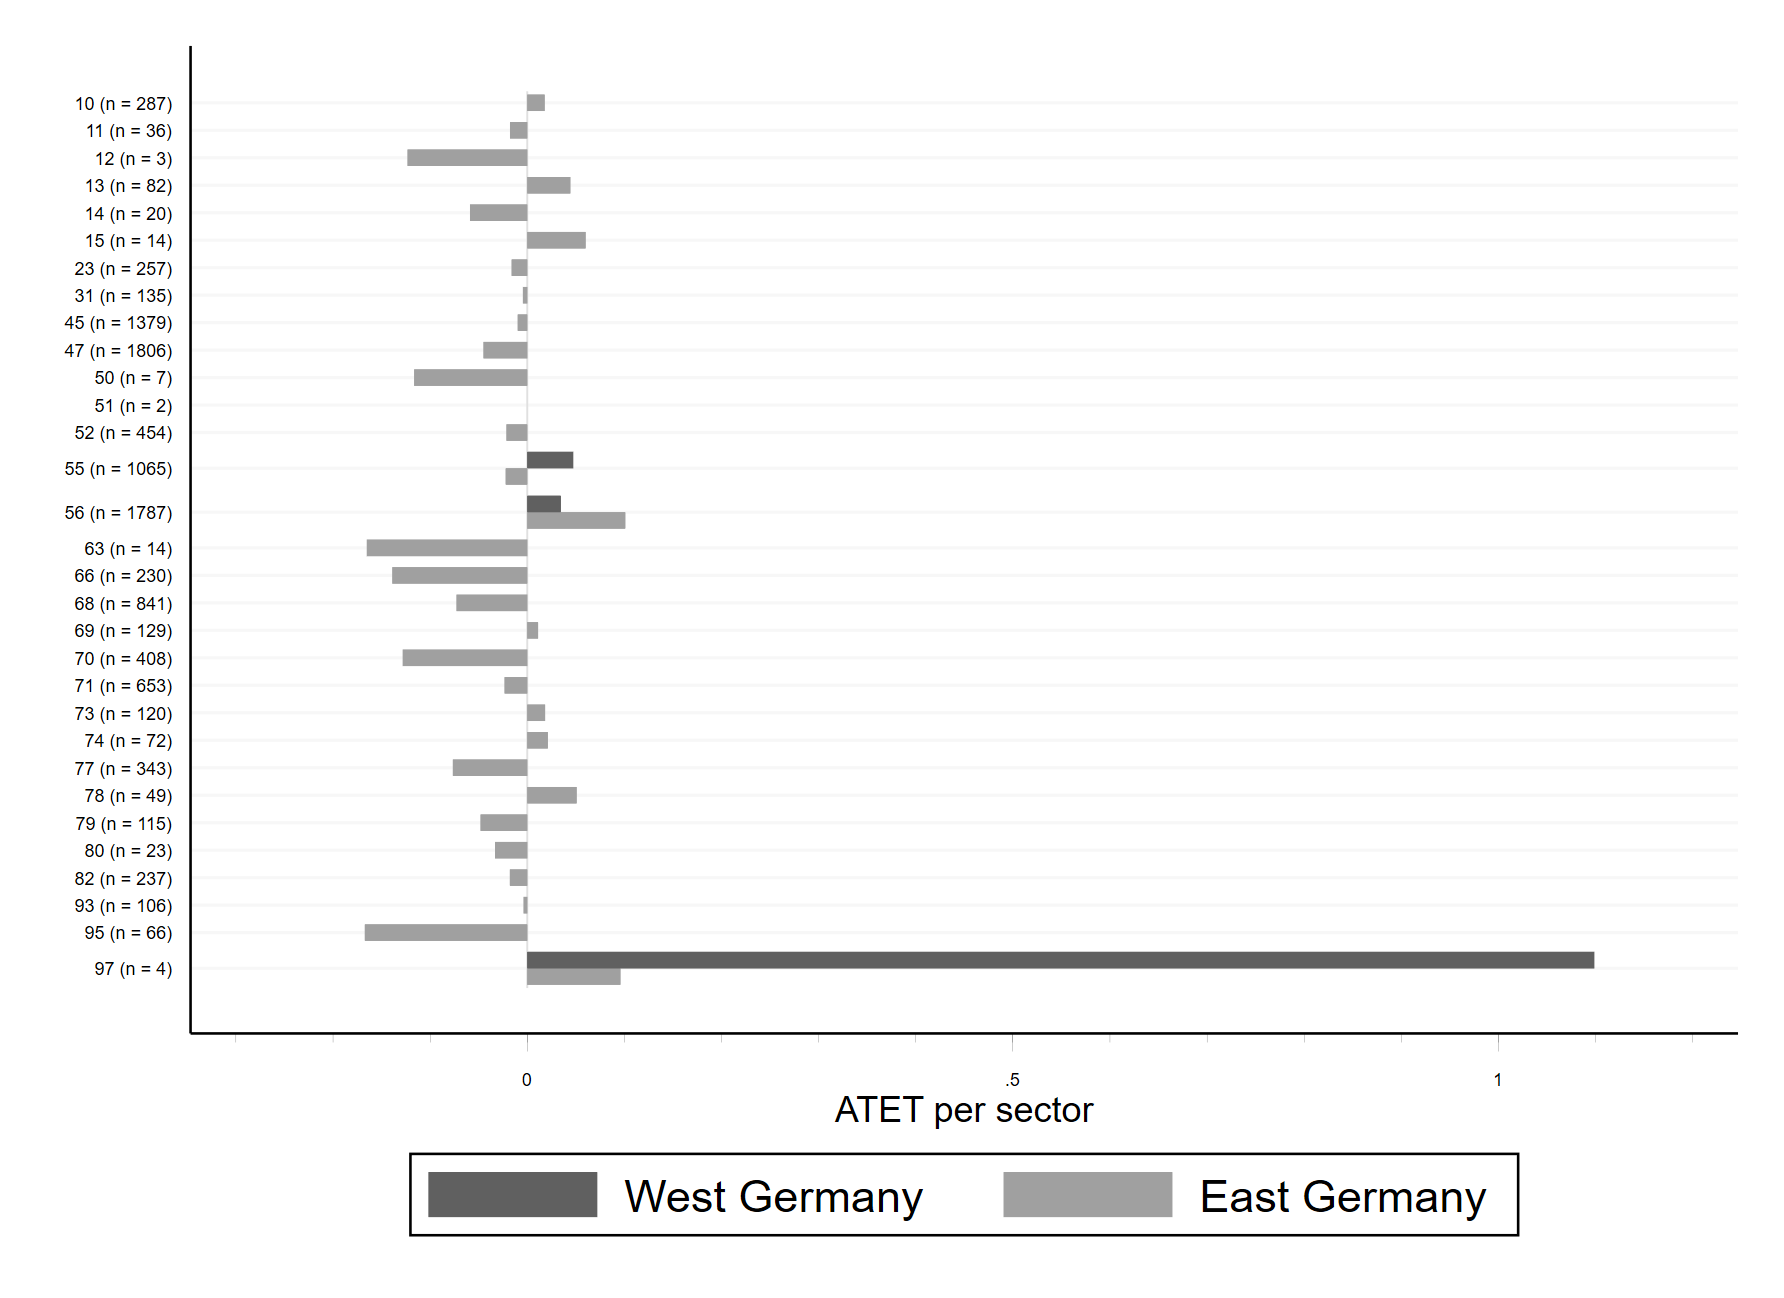
\includegraphics[width=0.70\paperwidth]{Images/ATET_per_sector_graph_ditor.png}
    \label{fig:sectorSplit}
\end{figure}